%
\chapter{Physical Properties of Low Temperature RF Plasmas}\label{sec:chapter_ccrfbasics}
%
	In this first chapter I will provide the necessary physical background for this work about the numerical simulation of low temperature capacitively coupled radio frequency plasmas. Here, both the simulation method as well as the most important aspects about the plasma properties will be introduced.
%
	\section{Plasma Physics}\label{sec:plasmaphysics}
%
		The experiment studied in this work is a capacitively coupled radio frequency (ccrf) discharge with a low temperature plasma, operated at low pressures. 
		A plasma is a globally quasi-neutral gas, consisting of freely moving charges --- e.g.\@ electrons, positive and negative ions --- with additional neutral gas particles. A plasma is characterised by the collective behaviour of the charged species. The ratio of charged particle density ($n\ix{i}$) and of the sum of neutral ($n\ix{n}$) and charged densities defines the \emph{degree of ionisation}. This is rather low for ccrf discharges, typically below 1\%.\\
		Charge separation of electrons and ions, and therefore the violation of the quasi-neutrality condition $n\ix{e}\,=\,n\ix{i}$ (electron density equals ion density), is only possible for distances below the \emph{Debye length} $\lambda\ix{D}$. Regions where the quasi-neutrality condition is satisfied are called plasma bulk. The definition of the degree of ionisation $\alpha$ and the Debye length are:
%
        \begin{align}
            \alpha=\frac{n\ix{i}}{n\ix{n}+n\ix{i}}\,,%
            \quad\text{~and~}\quad%
            \lambda\ix{D}^2&={\left(\lambda\ix{D,e}^{-2}+%
                \lambda\ix{D,i}^{-2}\right)}^{-1}\,.%
                \label{equ:degreeionizdebye}
        \end{align}
%		
        The creation of a plasma is accomplished by two parallel metal electrodes, where on at least one an ac or dc signal is applied. In this thesis I will consider alternating currents at radio frequency, $\SI{13.56}{\mega\hertz}$ with an amplitude between $100$--$\unit[1000]{V}$. A basic scheme of a radio frequency discharge can be seen in~\autoref{fig:circuitselfbias_1}. This asymmetric configuration, where the driven and grounded electrodes/walls are of different sizes is only one of many possible electric setups: coated or grounded electrodes are also possible, which create different operational regimes. In general, two driven metallic plates with an ionized working gas in between resemble a dielectric hindered plate capacitor. The neutral gas acts as a resistance and spatially restricted space-charges become dis-/chargeable capacities.\\
		The latter simplification can be used to understand important physical properties, such as an additional voltage offset on one of the electrodes or charge currents. For example: electrons are of a much smaller mass, which is why they are at least $\sqrt{m\ix{i}/m\ix{e}}$ -- times faster than the other species. Therefore they have a much higher mobility $\mu\ix{e}$ and thermal velocity $v\ix{th,e}$. Due to the fast response of the electron species, a plasma shields electric fields like by a short-circuit current.\\
		They also impinge onto walls more often, leading to the accumulation of a negative charge. Hence metal surfaces accumulate a negative potential bias due to the separation and higher mobility of the electrons. The same holds for electrodes with negative potential and grounded walls. Because charge conservation has to be satisfied, e.g. electron current onto the wall equals ion current, a spatially restricted area called \emph{plasma sheath} is established, where the electrons depletion occurs and ions are accelerated towards the wall.\\
		In the case of an asymmetric configuration with different electrode sizes, the potential inside the sheath can change drastically. This part of a plasma can have a huge impact on the behaviour of the discharge, e.g. an additional heating and energy dissipation into the plasma volume. Radio frequency plasmas are characterised by their transport process inside the sheath and heating mechanisms of charged species. A more in-depth discussion can be found in~\autoref{sec:heating}. The properties of the sheath are very important for plasma-assisted industrial applications, such as etching/sputtering and thin-film deposition.\\
    	An additional capacitance can be placed between electrode and generator. Such capacitively coupled rf discharges are characterised by a dc voltage offset on the electrode/s. This is called \emph{self bias} (see~\autoref{sec:selfbias}). The capacitor does not allow accumulated charges to flush to ground or the electric circuit. Furthermore, an additional current between plasma sheath and volume accommodates as a result of the different time scales of particle movement. This is called dielectric displacement current.\\
%		
        \vspace*{-0.5cm}
		\begin{wrapfigure}[18]{r}{0.4\textwidth}
			\centering
			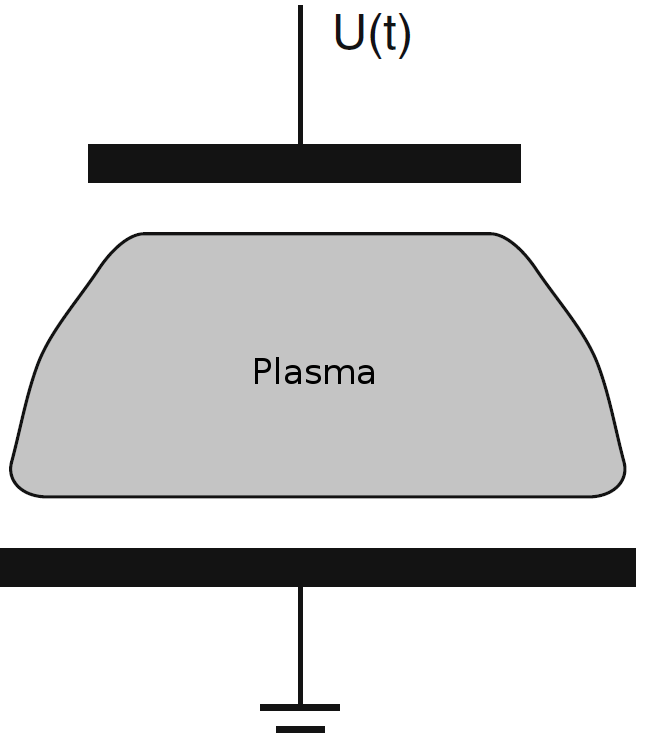
\includegraphics[width=0.35\textwidth]{figures/circuitselfbias_1.png}
			\caption{%
				Schematic of an asymmetric discharge with one grounded and %
			one driven electrode~\cite{Piel10}.}\label{fig:circuitselfbias_1}
		\end{wrapfigure}
%
        In this thesis we will exclusively consider oxygen as the working gas. An important aspect of oxygen plasmas, in contrast to most inert gases, is the creation of negative ions. One can define the property of \emph{electronegativity} $\eta$ as the ratio between anion and electron density: $\eta=n\ix{i-}/n\ix{e}$. The electronegativity can range between 0.03--4~\cite{Kullig12} in oxygen discharges of low temperatures and pressures.\\
        Negative ions affect the physics of the plasma volume. They behave like cold, heavy electrons and obey the same dynamic and kinetic laws. Collisions and processes involving negative ions heavily influence the discharge characteristics, e.g.\@ changing the distributions of the other species and thus create an ion-ion plasma, where electrons only form a peripheral plasma around the edges of the ion core.\\
        In the following section the interaction of plasma and walls will be highlighted, emphasising the difference in dynamics between electrons and ions.